\subsection{Konceptuālais datu bāzes apraksts}
Konceptuālajā modelī redzamās entītātes no konceptuālā ER modeļa (\ref{fig:conceptual-model} attēls):
\begin{itemize}
	\item Lietotājs - reģistrēts lietotājs, kas pieder noteiktai grupai;
	\item Attēls - datnes metadati un tās adrese, kas ir saistīta ar lietotāju vai spēles lomu;
	\item Maksas abonements - lietotāju maksas abonementa dati.
	\item Abonementa cena - cena par abonementu, kas darbojas noteiktā laika periodā.
	\item Spēles uzstādījums - vairāku spēles lomu kopa, kas ir izveidojamas arī publiski (maksas spēlētājiem)
	\item Spēles loma - spēlē izmantojamās lomas apraksts, katrai lomai obligāti piemīt trūkumi un darbības.
	      Tā var tikt izveidota publiski (analoģiski spēles uzstādījumiem);
	\item Lomas darbība - vienai vai vairākām spēles lomas piemītošās spēles darbības apraksts un spēlei specifiskie atribūti(/-s);
	\item Lomas trūkums - vienai vai vairākām spēles lomas piemītošā trūkuma apraksts;
	\item Spēlētājs - vienai virtuālai spēles istabai piederošais spēlētājs.
	      Tam piemīt viena spēles loma un var būt vairākas spēles gaitā veiktās
	      lomai atbilstošās darbības;
	\item Īsziņa - virtuālās istabas tērzēšanā izveidotā īsziņa, kas tiek saistīta ar vienu spēlētāju un var atbildēt uz citu īsziņu izveides laikā;
	\item Spēles notikums - spēles fāzes maiņa, spēlētāju izslēgšana, piemēram, izbalsošana vai slepkavība, un citi.
	\item Spēles virtuāla istaba - vienas gaidāmas, tekošās vai pagātnē notikušas spēles, kam piemīt spēlētāji, spēles uzstādījumi, spēles notikumi, izveidotājs (lietotājs maskas lietotāja grupā);
\end{itemize}

\begin{figure}[htbp]
	\centering
	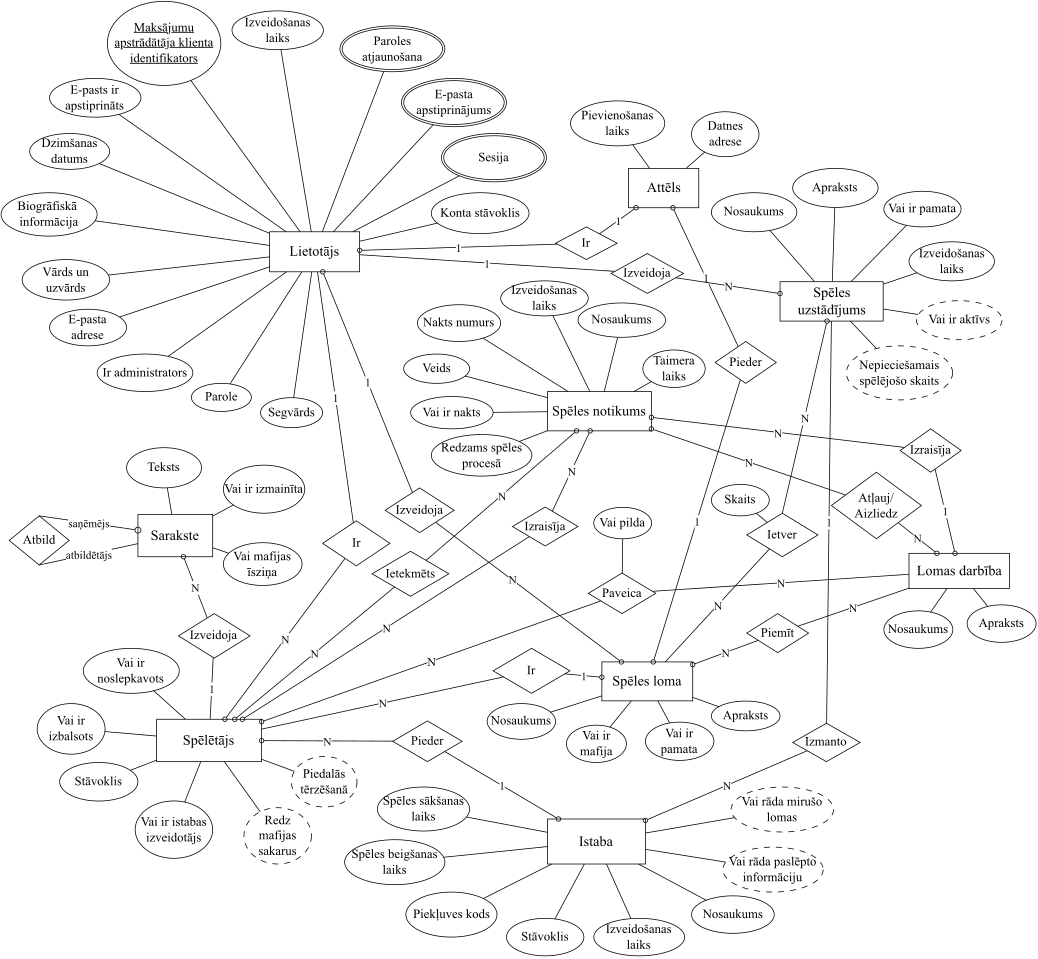
\includegraphics[width=\linewidth]{./src/img/KonceptualaisERModelis.png}
	\caption{Datu bāzes konceptuālais ER modelis}
	\label{fig:conceptual-model}
\end{figure}
